Information theory is very useful when analyzing the security of encryption schemes. Consider a scenario where one party, Alice wants to send a message $m$ (sampled from some random variable $M$) to another party, Bob, over some public channel, for example the internet. Alice and Bob share a key $k$ (sampled from another random variable $K$), which is a piece of information that is known only to them. Alice can use the key to encrypt her message (the \term{plaintext}), and Bob can use the same key to decrypt the \term{ciphertext} that Alice created, and read the message. The goal is to do this in such a way that if an eavesdropper (who usually goes by the name `Eve') listens in on the channel and intercepts the encrypted message, she cannot derive any information about the message as long as she does not know the key $k$.

\begin{center}
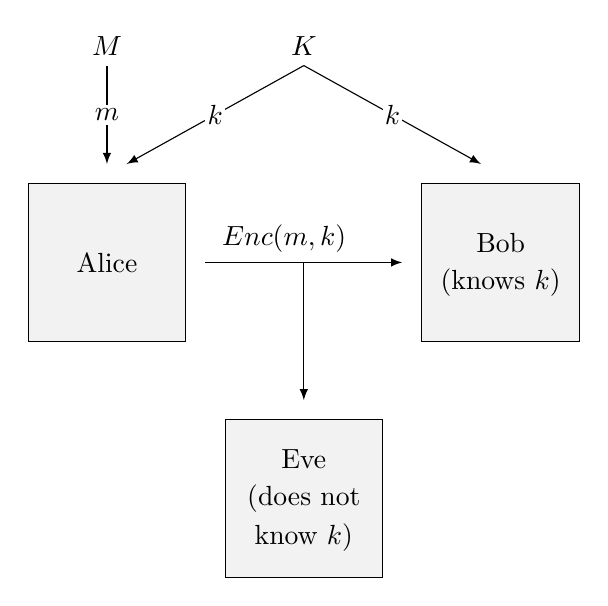
\begin{tikzpicture}
\draw[fill=black!5] (0,0) rectangle (2,2);
\draw[-latex] (2.25,1) -- (4.75,1);
%\draw[-latex,ocre,line width=2mm] (2.25,1) -- (4.75,1);
\draw[fill=black!5] (5,0) rectangle (7,2);
\node at (1,1) {Alice};
\node at (6,1.25) {Bob};
\node at (6,0.75) {(knows $k$)};
\node[anchor=south] at (3.25,1) {$Enc(m,k)$};

\draw[-latex] (1,3.5) -- (1,2.25);
\filldraw[fill=white,draw=none] (0.8,2.75) rectangle (1.2,3);
\node at (1,2.875) {$m$};
\node[anchor=south] at (1,3.5) {$M$};

\node[anchor=south] at (3.5,3.5) {$K$};
\draw[-latex] (3.5,3.5) -- (1.25,2.25);
\draw[-latex] (3.5,3.5) -- (5.75,2.25);
\filldraw[fill=white,draw=none] (2.25,2.75) rectangle (2.5,3);
\filldraw[fill=white,draw=none] (4.5,2.75) rectangle (4.75,3);
\node at (2.375,2.875) {$k$};
\node at (4.625,2.875) {$k$};

\draw[fill=black!5] (2.5,-3) rectangle (4.5,-1);
\node at (3.5,-1.5) {Eve};
\node at (3.5,-2) {(does not};
\node at (3.5,-2.5) {know $k$)};
\draw[-latex] (3.5,1) -- (3.5,-0.75);
%\draw[-latex, ocre,line width=1mm] plot [smooth,tension=0.5] coordinates {(2.25,0.95) (2.5,0.93) (3,0.75) (3.25,0.5) (3.5,0) (3.5,-0.75)};
\end{tikzpicture}
\end{center}

Let us formalize the above notion of encryption in the following definition:
\begin{definition}[Encryption scheme]\label{def:encryption}
An encryption scheme for (the message) $M$ consists of a key $K$ and a ciphertext $C = Enc(M,K)$, such that
\begin{itemize}
\item $I(M;K) = 0$ (the key is independent of the message -- this is a \term{setup assumption}), and
\item $H(M|KC) = 0$ (given the key and the ciphertext, Bob can recover the original message)
\end{itemize}
Note that $M$, $K$ and $C$ are random variables.
\end{definition}
Note that in order to satisfy the second requirement, the encryption function $Enc(\cdot,\cdot)$ needs to be injective: every message is mapped to a \emph{unique} ciphertext.


\section{Security}
Definition~\ref{def:encryption} does not put any constraints on the amount of information that Eve can get from the ciphertext: we still need to explicitly require the scheme to be secure.

\begin{definition}[Perfect security]
An encryption scheme is perfectly secure if
\[
I(M;C) = 0.
\]
This is equivalent to saying $H(M|C) = H(M)$, or to saying that $M$ and $C$ are independent.
\end{definition}
This type of security is also sometimes called perfect \term{information-theoric security}, in order to stress that the ciphertext really does not contain \emph{any} information about the plaintext message. Many commonly used encryption schemes do not provide this type of security. In \term{computationally secure} schemes, a lot of information about the message may be contained in the ciphertext, but it would take a ridiculous amount of resources (such as computation time or memory) to get the information out and derive the message.


\section{One-Time Pad}
A classic example of a perfectly secure encryption scheme is the one-time pad.

\begin{definition}[One-time pad]
Let the message space $\mathcal{M}$ be some additive group $(G,+)$. Define the random variable $K$ to be uniformly distributed over the key space $\mathcal{K} = \mathcal{M}$, and define the ciphertext space to be $\mathcal{C} = \mathcal{M}$ as well. Define the encryption and decryption function as follows:
\begin{align*}
Enc(m,k) &= m + k = c,\\
Dec(c,k) &= c + (-k) = m.
\end{align*}
Here, $c-k$ stands for $c + (-k)$, where $-k$ is the additive inverse of $k$.
\end{definition}
\begin{example}[One-time pad for binary strings]
The most common use of the one-time pad is for the group of binary strings under addition modulo 2, i.e.\ $(\{0,1\}^n, \oplus)$. In this group, every element is its own additive inverse, resulting in the encryption and decryption functions
\begin{align*}
Enc(m,k) &= m \oplus k = c,\\
Dec(c,k) &= c \oplus k = m.
\end{align*}
For example, if $n=4$, a possible message $m$ is 0101, and a possible key $k$ is 0110. The ciphertext $c$ is $0101 \oplus 0110 = 0011$, and the decryption of $c$ is again $0011 \oplus 0110 = 0101$, the original message $m$.
\end{example}
We can show that the one-time pad indeed satisfies the security definition of the previous section.
\begin{theorem}
The one-time pad is perfectly secure.
\end{theorem}
\begin{proof}
Write $n = \log|G|$. We need to verify that $I(M;C) = 0$. We do so using a three-variable entropy diagram (see Section~\ref{sec:Venn}). We can already fill in the values $H(K) = n$ (because $K$ is uniformly distributed), $H(M|CK) = H(C|MK) = H(K|MC) = 0$ (because each random variable is a function of the other two), and $I(M;K) = 0$ (this is our setup assumption). Write $n = \log|G|$ in the diagram:

\begin{center}
\begin{tikzpicture}
\def\size{1.5}
\def\circleA{(0,0) circle (\size cm)} %top left
\def\circleB{(\size,0) circle (\size cm)} %top right
\def\circleC{(\size/2,-\size) circle (\size cm)} %bottom
\fill[black!5] \circleA;
\fill[black!5] \circleB;
\fill[black!5] \circleC;
\begin{scope}
\clip\circleA;
\fill[white] \circleB;
\end{scope}
\begin{scope}
\clip\circleB;
\fill[white] \circleC;
\end{scope}
\begin{scope}
\clip\circleA;
\fill[ocre!50] \circleC;
\end{scope}
\draw\circleA;
\draw\circleB;
\draw[line width=1mm]\circleC;
\node at (-\size/2,\size/8) {0};
\node at (\size+\size/2,\size/8) {0};
\node at (\size/2,\size/3) {};
\node at (\size/2,-1.4*\size) {0};
\node at (-\size/2,\size + 0.1) {$H(M)$};
\node at (\size*1.5,\size + 0.1) {$H(C)$};
\node at (-0.1*\size,-0.65*\size) {$a$};
\node at (1.1*\size,-0.65*\size) {$n$};
\node at (\size/2,-0.4*\size) {$-a$};
\node at (\size/2,-2.3*\size) {$H(K) = n$};
\end{tikzpicture}
\end{center}
Note that the area of $I(M;K) = I(M;K|C) + R(M;K;C)$ (shaded orange in the picture) as a whole is 0, but that does not mean that $I(M;K|C)$ and $R(M;K;C)$ themselves are zero, because $R(M;K;C)$ can be negative. We can conclude that there must be some (non-negative) real number $a$ such that $I(M;K|C) = a$ and $R(M;K;C) = -a$. From the diagram, we can furthermore conclude that $I(K;C|M) = n$.

We now argue that $H(C) = n$. We do so by showing that $P_C(c) = \frac{1}{|G|}$ for arbitrary $c$: \yfke{or is there a nice way to see this from the diagram?}
\begin{align}
P_C(c) &= \sum_{m \in \mathcal{M}} P_{MC}(m,c)\nonumber\\
&= \sum_{m \in \mathcal{M}} P_M(m) P_{C|M}(c|m)\nonumber\\
&= \sum_{m \in \mathcal{M}} P_M(m) \left(\sum_{k \in \mathcal{K}} P_{CK|M}(c,k|m)\right)\nonumber\\
&= \sum_{m \in \mathcal{M}} P_M(m) \left(\sum_{k \in \mathcal{K}} P_{K|M}(k|m) P_{C|KM}(c|k,m)\right)
\end{align}
Since also $K$ and $M$ are independent (the setup assumption) and hence $P_{K|M}(k|m) = P_K(k)$ for all $k \in \mathcal{K}$,
\begin{align}
P_C(c) = \sum_{m \in \mathcal{M}} P_M(m) \left(\sum_{k \in \mathcal{K}} P_{K}(k) P_{C|KM}(c|k,m)\right)
\end{align}
Note that $P_{C|KM}(c|k,m) = 1$ if $c = k + m$, and 0 otherwise. We can thus continue the computation by
\begin{align}
P_C(c) &= \sum_{m \in \mathcal{M}} P_M(m) P_K(c - m)\nonumber\\
&= \sum_{m \in \mathcal{M}} P_M(m) \frac{1}{|G|}\nonumber\\
&= \frac{1}{|G|}
\end{align}
Incorporating the fact that $H(C) = n$ in our entroy diagram, we see that $(M;C|K) = a$, and the total mutual information $I(M;C) = 0$, as desired:
\begin{center}
\begin{tikzpicture}
\def\size{1.5}
\def\circleA{(0,0) circle (\size cm)} %top left
\def\circleB{(\size,0) circle (\size cm)} %top right
\def\circleC{(\size/2,-\size) circle (\size cm)} %bottom
\fill[black!5] \circleA;
\fill[black!5] \circleB;
\fill[black!5] \circleC;
\begin{scope}
\clip\circleB;
\fill[white] \circleC;
\end{scope}
\begin{scope}
\clip\circleA;
\fill[white] \circleC;
\end{scope}
\begin{scope}
\clip\circleA;
\fill[ocre!50] \circleB;
\end{scope}
\draw\circleA;
\draw[line width=1mm]\circleB;
\draw\circleC;
\node at (-\size/2,\size/8) {0};
\node at (\size+\size/2,\size/8) {0};
\node at (\size/2,\size/3) {$a$};
\node at (\size/2,-1.4*\size) {0};
\node at (-\size/2,\size + 0.1) {$H(M)$};
\node at (\size*1.5,\size + 0.1) {$H(C) = n$};
\node at (-0.1*\size,-0.65*\size) {$a$};
\node at (1.1*\size,-0.65*\size) {$n$};
\node at (\size/2,-0.4*\size) {$-a$};
\node at (\size/2,-2.3*\size) {$H(K) = n$};
\end{tikzpicture}
\end{center}


\end{proof}
We have thus seen that the one-time pad provides perfect information-theoretic security. There is one practical drawback to this encryption scheme though: the key needs to be as large as the message! To send a message of $n$ bits, Alice needs to share $n$ bits of key with Bob. It might be tempting for Alice to reuse the key $k$ for several messages once she has shared it with Bob, but this is dangerous: Eve could, from two intercepted encryptions $(m_1 + k)$ and $(m_2 + k)$, recover the encryption $m_1 + k - m_2 - k = m_1 - m_2$. Even the difference between two plaintext messages can already reveal a lot of information about the individual messages, as illustrated in \href{https://cryptosmith.com/2008/05/31/stream-reuse/}{this Cryptosmith blog post}.

\section{Minimum Key Length}
It turns out to be impossible to design an encryption scheme that provides both perfect security and short keys. So even though the one-time pad may seem inefficient, its key lengths are optimal for a perfectly secure scheme.
\begin{theorem}
For any perfectly secure encryption scheme, it holds that $H(K) \geq H(M)$.
\end{theorem}
\begin{proof}
Again, we turn to entropy diagrams. Write $a = I(M;C|K) \geq 0$. using the fact that $I(M;K) = 0$ (setup assumption) and $I(M;C) = 0$ (security), we can fill in the entropy diagram as follows:

\begin{center}
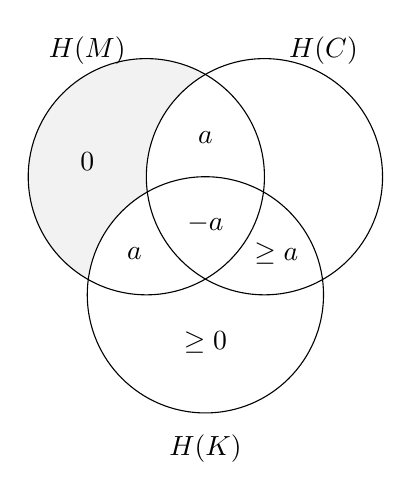
\begin{tikzpicture}
\def\size{1.5}
\def\circleA{(0,0) circle (\size cm)} %top left
\def\circleB{(\size,0) circle (\size cm)} %top right
\def\circleC{(\size/2,-\size) circle (\size cm)} %bottom
\fill[black!5] \circleA;
\begin{scope}
\clip\circleA;
\fill[white] \circleB;
\end{scope}
\begin{scope}
\clip\circleA;
\fill[white] \circleC;
\end{scope}
\draw\circleA;
\draw\circleB;
\draw\circleC;
\node at (-\size/2,\size/8) {0};
\node at (\size+\size/2,\size/8) {};
\node at (\size/2,\size/3) {$a$};
\node at (\size/2,-1.4*\size) {$\geq 0$};
\node at (-\size/2,\size + 0.1) {$H(M)$};
\node at (\size*1.5,\size + 0.1) {$H(C)$};
\node at (-0.1*\size,-0.65*\size) {$a$};
\node at (1.1*\size,-0.65*\size) {$\geq a$};
\node at (\size/2,-0.4*\size) {$-a$};
\node at (\size/2,-2.3*\size) {$H(K)$};
\end{tikzpicture}
\end{center}
Note that $I(K;C|M) \geq a$ follows from the fact that $I(C;K) \geq 0$ and $R(C;K;M) = -a$.

From the diagram, we observe that $H(M) = a$, and that $H(K) \geq a$. Hence, $H(K) \geq H(M)$.
\end{proof}